\documentclass[language=german,style=solution]{smo}

\usepackage{tikz}
\usetikzlibrary{patterns}
\usetikzlibrary{decorations.pathreplacing}

\examplace{Zürich}
\examdate{7./8./21./22. Mai 2016}

\title{IMO-Selektion - Musterlösung}

\begin{document}

\begin{enumerate}

\item[\textbf{1.}] %% Exercise 1 %%
Sei $n$ eine natürliche Zahl. Wir nennen ein Zahlenpaar \emph{unverträglich}, falls ihr grösster gemeinsamer Teiler gleich 1 ist. Wie viele unverträgliche Paare treten mindestens auf, wenn man die Zahlen $\{1, 2, \ldots, 2n\}$ in $n$ Paare aufteilt?

\textit{Lösung (Viviane):}
Wir nennen ein nicht unverträgliches Paar \emph{verträglich}. Es ist klar, dass Primzahlen strikt grösser als $n$ Teil eines unverträglichen Paars sind, und $1$ ebenfalls Teil eines unverträglichen Paars ist. Also gibt es wegen diesen Zahlen mindestens
\[
	\left\lceil\frac{\text{(Anzahl Primzahlen zwischen }n \text{ und }2n) + 1}{2}\right\rceil
\]
unverträgliche Paare. Wir teilen diese Menge in unverträgliche Paare auf. Falls diese Menge eine ungerade Anzahl Zahlen hat, teilen wir die letzte Zahl mit $2$ in ein unverträgliches Paar ein.

 Wir zeigen, dass wir die restlichen Zahlen in verträgliche Paare aufteilen können. Dazu betrachte nacheinander die ungeraden Primzahlen $p_1<p_2<\ldots<p_r\leq n$. Betrachte nun nacheinander die Menge der noch übrigen Zahlen, die durch $p_i$ teilbar sind. Falls diese Menge eine gerade Anzahl Elemente hat, teile sie in per Konstruktion verträgliche Paare auf. Falls diese Menge eine ungerade Anzahl Elemente hat, wähle ein gerades Element in der Menge. Dieses existiert, da $2p_i$ sicher in der Menge liegt. Teile die restlichen Elemente der Menge in Paare auf. Wenn wir alle Primzahlen betrachtet haben, bleiben also eine gerade Anzahl Zahlen übrig, da wir immer paarweise Zahlen weggenommen haben. Diese sind alle gerade, also können wir sie in verträgliche Paare aufteilen.
 
\textit{Marking Scheme:}
\begin{itemize}
\item Das finden und korrekte Begründen der unteren Schranke
\[
	\left\lceil\frac{\text{(Anzahl Primzahlen zwischen }n \text{ und }2n) + 1}{2}\right\rceil
\]
gibt 2 Punkte.
\item Eine korrekte Konstruktion, welche diese Schranke tatsächlich realisiert, ist 5 Punkte wert. 
\item Wenn die Konstruktion einen Fehler enthält, welcher sich einfach und mit den bereits vorhandenen Ideen beheben lässt, können, entsprechend dem Schweregrad des Fehlers, Teilpunkte erhalten werden.
\end{itemize}


\newpage

\item[\textbf{2.}] %% Exercise 2 %%
Finde alle Polynome $P$ mit reellen Koeffizienten, sodass folgende Gleichung für alle $x \in \R$ gilt:
\[
(x-2)P(x+2)+(x+2)P(x-2)=2xP(x).
\]

\textit{Lösung (Viviane):}\\
Einsetzen von $x=0$ und $x=2$ liefert $P(-2)=P(0)=P(2)$, also können wir $P(x)$ schreiben als $Q(x)(x-2)(x)(x+2)+a$. Einsetzen in die ursprüngliche Gleichung liefert
\[
(x-4)Q(x-2)+(x+4)Q(x+2)=2xQ(x).
\]
Falls wir ein $s<4$ finden, sodass $Q(s)=Q(s+2)=k$, dann folgt
\[
Q(s-2)=\frac{2sk-(s+4)k}{s-4}=k.
\]
Induktiv folgt dann $Q(s-2n)=k$, somit ist $Q$ konstant.
Einsetzen von $x=-4$ in obige Gleichung liefert $Q(-6)=Q(-4)$. Da $-6<4$ ist, ist $Q$ somit konstant. Einsetzen liefert, dass
\[
P(x)=b(x-2)(x)(x+2)+a
\]
auch tatsächlich Lösungen sind.

\textit{Marking Scheme:}
\begin{itemize}
\item $P(x)=Q(x)x(x-2)(x+2)+a$ 2 Punkte
\item Q konstant oder irgendwie Grad von $P$ sinnvoll beschränken: insgesamt 5 Punkte
\item fertigmachen: 2 Punkte
\end{itemize}
\newpage

\item[\textbf{3.}] %% Exercise 3 %%
Sei $ABC$ ein Dreieck mit $\angle BCA = 90^\circ$ und $H$ der Höhenfusspunkt von $C$. Sei $D$ ein Punkt innerhalb des Dreiecks $BCH$, sodass $CH$ die Strecke $AD$ halbiert. Sei $P$ der Schnittpunkt der Geraden $BD$ und $CH$. Sei $\omega$ der Halbkreis mit Durchmesser $BD$, der die Strecke $CB$ schneidet. Die Tangente von $P$ an $\omega$ berühre diesen in $Q$. Zeige, dass der Schnittpunkt der Geraden $CQ$ und $AD$ auf $\omega$ liegt.

\textit{Lösung (Cyril):}\\
Sei $K$ die Projektion von $D$ auf $AB$. Dann gilt $AH = HK$. Da. $PH \parallel DK$ haben wir
\[
\frac{PD}{PB} = \frac{HK}{HB} =  \frac{AH}{HB}
\]
Sei $L$ die Projektion von $Q$ auf $DB$. Da $PQ$ die Tangente and $\omega$ ist, und $\angle DQB = \angle BLQ = 90^\circ$, folgt $\angle PQD = \angle QBP = \angle DQL$. Damit sind $QD$ und $QB$ die (innere bzw. äussere) Winkelhalbierende von $\angle PQL$. Nach dem Winkelhalbierendensatz folgt
\[
\frac{PD}{DL} =  \frac{PQ}{QL} = \frac{PB}{BL}.
\]

Diese zwei Gleichungen ergeben zusammen:
\[
\frac{AH}{HB} = \frac{DL}{LB}.
\]
Dies bedeutet, dass wir den grossen Halbkreis so um $B$ drehen und strecken können, sodass dieser auf $\omega$ liegt und dabei $A$ auf $D$ und $H$ auf $L$ abgebildet wird. Da wir jeweils die Senkrechte zu $H$ bzw. $L$ nehmen, wird $C$ auf $Q$ abgebildet.

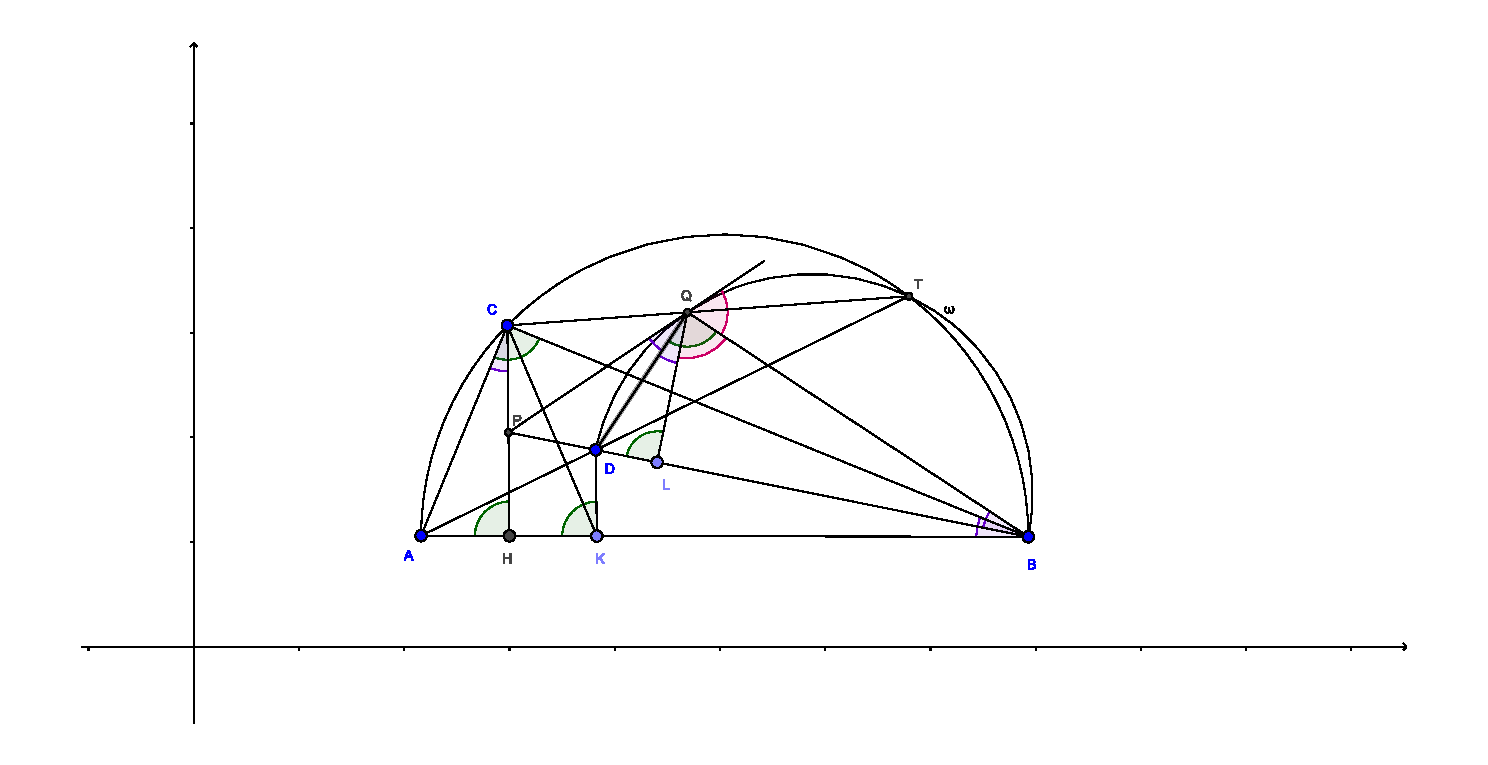
\includegraphics[width=\textwidth, trim=6cm 3cm 7cm 3cm, clip=true]{graphics/2016_3.pdf}

Daraus bekommen wir das Verhältnis
\[
\frac{AB}{BD} = \frac{CB}{BQ}
\]
und den Winkel
\[
\angle ABD = \angle CBQ
\]
Dies zusammen führt, dass die Dreieck $ABD$ und $CBQ$ ähnlich sind und daher $\angle BDT = \angle BQT$. ($T$ sei der Schnittpunkt der Gerade $CQ$ und $AD$) Nach der Umkehrung des Peripheriewinkels liegt $T$ auf $\omega$.

\textit{Marking Scheme}
\begin{itemize}
\item 4 Punkte bis $ABD$ und $CBQ$ ähnlich
\end{itemize}


\newpage


\item[\textbf{4.}] %% Exercise 4 %%

Bestimme alle natürlichen Zahlen $n$, sodass für beliebige reelle Zahlen $x_1, \ldots, x_n$ gilt:
\[
\left(\frac{x_1^n + \ldots + x_n^n}{n} - x_1\cdot \ldots \cdot x_n\right) \left(x_1 + \ldots + x_n \right)  \geq 0.
\]

\textit{Lösung (Vivi und Jana):}
Für eins geht es trivialerweise. Die Ungleichung ist für drei erfüllt. Die Ungleichung lässt sich wie folgt faktorisieren:
\[
\frac{1}{6} (x_1+x_2+x_3)^2((x_1-x_2)^2+(x_2-x_3)^2+(x_3-x_1)^2)\geq 0.
\]
Für alle anderen Zahlen geht es nicht. Wir geben Gegenbeispiele:
\begin{itemize}
\item $n=2$: $x_1=0, x_2=-1$.
\item $n>3$: $x_1=x_2=-2, x_3=3, x_4=\ldots=x_n=0$. Da die zweite Klammer $-1$ ist, müssen wir noch zeigen, dass die erste Klammer positiv ist. Diese ist von der Form 
\[
\left(\frac{(-2)^n + (-2)^n+3^n+0^n+ \ldots + 0^n}{n} - (-2)\cdot(-2)\cdot3\cdot \ldots\cdot0\right)=\frac{2\cdot(-2)^n+3^n}{n}.
\]
Ausklammern führt zu 
\[
\frac{8\cdot(-2)^{n-2}+9\cdot3^{n-2}}{n}.
\]
Für $n\geq2$ ist dies positiv.
\end{itemize}

\textit{Marking Scheme:}
\begin{itemize}
\item Der Fall $n=3$ gibt 3 Punkte.
\item Für eine obere Schranke gibt 1 Punkt.
\item Die restlichen Fälle geben 3 Punkte, wobei jeder vergessene Fall 1~Punkt Abzug gibt.

%\item Eine obere Schranke für mögliche $n$ gibt 1 Punkt.
%\item Vergessene Fälle geben $-1$ Punkt.
\end{itemize}


\newpage

\selectlanguage{french}

\item[\textbf{5.}] %% Exercise 5 %%

Soit $A$ un ensemble fini de nombres naturels. Une partition de $A$ en deux sous-ensembles disjoints non-vides $A_1$ et $A_2$ est appelée \emph{démoniaque} si le plus petit multiple commun des éléments de $A_1$ est égal au plus grand diviseur commun des éléments de $A_2$. Quel est le plus petit nombre d'éléments que $A$ doit avoir pour qu'il existe exactement 2016 partitions démoniaques?

\textit{Solution (Louis): }
Soit $A = A_1 \cup A_2$ une partition démoniaque et soient $a = \max{(A_1)}$, $b = \min{(A_2)}$. On a alors que le plus petit multiple commun des éléments de $A_1$ est plus grand ou égal à $a$ et le plus grand diviseur commun des éléments de $A_2$ est plus petit ou égal à $b$. Il faut donc que $a < b$, et ainsi $A_1$ et $A_2$ sont obtenus à partir de $A$ en mettant tous les éléments inférieurs à un certain nombre dans $A_1$ et tous les éléments restants dans $A_2$. En particulier, si $A$ possède $n$ éléments, le nombre de partitions démoniaques vaut au plus $n-1$.

 Construisons maintenant un ensemble $A$ qui admet exactement $2016$ partitions démoniaques. On écrit la paire $(x, y)$ pour représenter le nombre $2^x\cdot 3^y$ et l'ensemble $A$ est alors
\[
 	A = \frack{(0,0), (1,0), (0,1), (1,1), (2,1), (1,2), (2,2), \ldots, (1008, 1008)}.
\]
On voit facilement que l'on peut mettre la séparation entre $(a, a)$ et $(a+1, a)$ ou entre $(a,a+1)$ et $(a+1, a+1)$ pour obtenir des ensembles démoniaques. Cela donne alors exactement $2016$ ensembles démoniaques et $A$ possède $3025$ éléments.

Il reste à montrer que $A$ doit forcément avoir au moins $3025$ éléments. Pour fixer la notation, soit 
\[
	A = \frack{x_1, x_2, \ldots, x_n}.
\]
Tout d'abord on ne peut pas avoir que $A_1 = \frack{x_1}$ et $A'_1 = \frack{x_1, x_2}$ soient deux partitions démoniaques. En effet si $A_1, A_2$ est une partition démoniaque, le ppmc de $A_1$ vaut $x_1$ et donc le pgcd de $A_2$ également, donc $x_1\div x_i$ pour tout $i\geq 1$. En particulier $x_1\div x_2$ donc le ppmc de $A'_1$ vaut $x_2$, ce qui implique que le pgdc de $A'_2$ vaut $x_2$ et donc $x_2\div x_i$ pour tout $i\geq 2$. Mais alors le pgdc de $A_2$ est $x_2$, ce qui contredit le fait que $A_1, A_2$ est une partition démoniaque.
Supposons qu'il existe $i$ tel que $A_1 = \frack{\ldots, x_i}, A'_1 = \frack{\ldots, x_i, x_{i+1}}, A''_1 = \frack{\ldots, x_i, x_{i+1}, x_{i+2}}$ forment trois partitions démoniaques. Nous avons alors les relations
\[
	x_i \div ppmc(A_1) = pgdc(A_2) \div b\quad \forall b\in A_2
\]\[
	x_{i+1} \div ppmc(A'_1) = pgdc(A'_2) \div b'\quad \forall b'\in A'_2
\] et \[
	x_{i+2} \div ppmc(A''_1) = pgdc(A''_2) \div b''\quad \forall b''\in A''_2.
\]
Cependant les deux dernières relations impliquent alors que $pgdc(A'_2) = x_{i+2}$ et $pgdc(A_2) = x_{i+1}$, et donc également que $ppmc(A_1) = x_{i+1}$ car $A_1, A_2$ est démoniaque. Nous arrivons maintenant à une contradiction car $A'_1$  est construit en rajoutant à $A_1$ uniquement l'élément $x_{i+1}$, donc $ppmc(A'_1) = x_{i+1}$ également, et comme on a déjà prouvé que $pgdc(A'_2) = x_{i+2}$ la paire $A'_1, A'_2$ ne pourrait être démoniaque. Ainsi il est impossible d'obtenir $2016$ paires démoniaques si $A$ possède strictement moins de $3025$ éléments.

\textit{Marking Scheme:}
\begin{itemize}
\item $\abs{A} \leq 3025$: 3 points
\item $\abs{A} \geq 3025$: 4 points, dont un point si l'on prouve qu'il suffit de considérer les $\abs{A}-1$ partitions données en séparant les plus petits éléments des plus grands.
\item Si l'argument est correct mais le nombre d'éléments calculé est faux: -1 point
\end{itemize}

\selectlanguage{ngerman}

\newpage

\item[\textbf{6.}] %% Exercise 6 %%

Sei $n$ eine natürliche Zahl. Zeige, dass $7^{7^{n}}+1$ mindestens $2n+3$ nicht notwendigerweise verschiedene Primteiler hat.

\textit{Bemerkung: $18 = 2\cdot 3\cdot 3$ hat 3 Primteiler.}

\textit{Lösung (Paul und Fabian):}

Wir lösen das Problem per Induktion. Die Verankerung ist der Fall $n = 0$, bei dem $7^{7^0} + 1 = 7^1 + 1 = 2^3$ gilt. Für den Induktionsschritt gilt es zu zeigen, dass wenn $x = 7^{2m - 1}$ für eine natürliche Zahl $m$ gilt, dass $(x^7 + 1)/(x + 1)$ nicht prim ist. Daraus folgt, dass $x^7 + 1$ mindestens zwei Primteiler mehr hat als  $x + 1$. Wir zeigen nun, dass $(x^7 + 1)/(x + 1)$ nicht prim ist:
\begin{align*}
\frac{x^7 + 1}{x + 1} &= \frac{(x + 1)^7 - ((x + 1)^7 - (x^7 + 1))}{x + 1} \\
&= (x + 1)^6 - \frac{7x(x^5 + 3x^4 + 5x^3 + 5x^2 + 3x + 1)}{x + 1} \\
&= (x + 1)^6 - 7x(x^4 + 2x^3 + 3x^2 + 2x + 1) \\
&= (x + 1)^6 - 7^{2m}(x^2 + x + 1)^2 \\
&= \{(x + 1)^3 - 7^m(x^2 + x + 1)\}\{(x + 1)^3 + 7^m(x^2 + x + 1)\}.
\end{align*}
Nun gilt es noch zu zeigen, dass beide Faktoren grösser als 1 sind. Es reicht, dies für den kleineren zu zeigen. Mit $\sqrt{7x}\leq x$ folgt:
\begin{align*}
(x + 1)^3 - 7^m(x^2 + x + 1) &= (x + 1)^3 - \sqrt{7x}(x^2 + x + 1) \\
&\geq x^3 + 3x^2 + 3x + 1 - x(x^2 + x + 1) \\
&= 2x^2 + 2x + 1\geq 113 > 1.
\end{align*}
Also ist $(x^7 + 1)/(x + 1)$ nicht prim und die Aussage ist bewiesen.

\textit{Marking Scheme:}
\begin{itemize}
\item 3 Punkte für die Faktorisierung.
\item 3 Punkte wenn man fertig wird.
\end{itemize}

\newpage

\item[\textbf{7.}] %% Exercise 7 %%
Finde alle natürlichen Zahlen $n$, sodass gilt:
\[
\sum_{\substack{d\div n\\ 1\leq d < n}} d^2=5(n+1).
\]

\textit{Lösung (Viviane):}
Wir betrachten $n$ gerade und $n$ ungerade einzeln.

Fall 1: $n$ ist gerade:\\
$n$ kann nicht 2 sein. Falls $n>2$ ist, hat $n$ die Teiler $1, 2$ und $n/2$. Es folgt, dass $1+4+(n/2)^2\leq 5(n+1)$. Umformen liefert $n\leq20$. Durchtesten der Fälle ergibt die Lösung $n=16$.

Fall 2: $n$ ist ungerade:\\
Eins ist keine Lösung. Die rechte Seite ist gerade, also auch die linke Seite. Alle Teiler von $n$ sind ungerade. Es folgt, dass $n$ eine ungerade Anzahl Teiler (mit sich selbst) hat, also ist $n$ eine Quadratzahl. Potenzen ungerader Primzahlen sind keine Lösungen, denn dann ist die linke Seite $\equiv1$ modulo $p$ und die rechte Seite $\equiv 5 \mod p$. Dies funktioniert nur, falls $0\equiv4 \mod p$, also $p=2$, also $n$ gerade.\\
Somit können wir $n=(ps)^2$ schreiben, wobei $p$ dem kleinsten Primteiler von $n$ ist und $s$ mindestens ein Primteiler $\neq p$ besitzt. Es folgt, dass $n$ die drei verschiedenen Teiler $1,p$ und $ps^2$ besitzt. Ausserdem sind $p$ und $s$ ungerade und nicht eins, somit sind beide grösser als 2. Also muss gelten
\[
5+9(ps)^2=1+4+9(ps)^2\leq 1+p^2+s^2(ps)^2\leq5((ps)^2+1),
\]
was nicht möglich ist.

Also ist $n=16$ die einzige Lösung.

Weitere Lösungen sind zum Beispiel, wenn man zuerst die Anzahl Teiler gegen oben begrenzt und dann Fallunterscheidungen macht, oder wenn man die Anzahl verschiedene Primteiler abschätzt und dann Fallunterscheidungen macht.


\textit{Marking Scheme:}
Punkte verschiedener Lösungswege sind nicht additiv, man bekommt Punkte für den Lösungsweg, wo man am weitesten gekommen ist.
\begin{itemize}
	\item Punkte für MuLö:
	\begin{itemize}
		\item$n$ gerade: 1 Punkt für $n\leq20$, dann 1 Punkt für $n=16$.
		\item$n$ ungerade: 1 Punkt für $n$ Quadratzahl, dann 1 Punkt für $n$ keine Primpotenz, 5 Punkte, 					wenn Fall $n$ ungerade insgesamt.
	\end{itemize}
 	\item Punkte, wenn man Anzahl Teiler abschätzt:
 	\begin{itemize}
 		\item weniger als 16 Teiler: 1 Punkt
 		\item weniger als 8 Teiler: 2 Punkte (nicht additiv zu 1 Punkt)
 		\item $n$ keine Primpotenz: 1 Punkt
 	\end{itemize}
 	\item Punkte, wenn man Primteiler abschätzt:
 	\begin{itemize}
 		\item $n$ keine Primpotenz: 1 Punkt
 		\item $n$ zwei verschiedene Primteiler: 3 Punkte
 		\item $n$ mehr als zwei verschiedene Primteiler: 2 Punkte
 	\end{itemize}
\end{itemize}

\newpage

\item[\textbf{8.}] %% Exercise 8 %%

Soit $ABC$ un triangle avec $AB\neq AC$ et soit $M$ le milieu de $BC$. La bissectrice de $\angle BAC$ coupe la droite $BC$ en $Q$. Soit $H$ le pied de la hauteur en $A$ sur $BC$. La perpendiculaire à $AQ$ passant par $A$ coupe la droite $BC$ en $S$. Montrer que $MH\cdot QS = AB \cdot AC$.

\textit{Solution (Horace):}\\
Soit $I$ le point d'intersection de la médiatrice de $BC$ et de la bissectrice de $\angle BAC$. Celui-ci est bien défini car $AB\neq AC$. Il est connu que la bissectrice d'un angle d'un triangle et la médiatrice du coté opposé s'intersectent sur le cercle circonscrit du triangle. De là s'ensuit que $A$,$B$,$C$ et $I$ sont sur un cercle. Du ce fait, on déduit que $\angle ACB= \angle IAB$. Comme par construction $AI$ bissecte $\angle BAC$, on a $\angle IAC=\angle AIB$. De ces deux dernières égalités on a que $ACQ$ et $AIB$ sont semblables. De cette similarité on tire le premier résultat important:
\[
\frac{AC}{AQ}=\frac{AI}{AB}
\]
et par conséquent,
\begin{equation}
	AB \cdot AC=AI \cdot AQ \label{eq:un}
\end{equation}

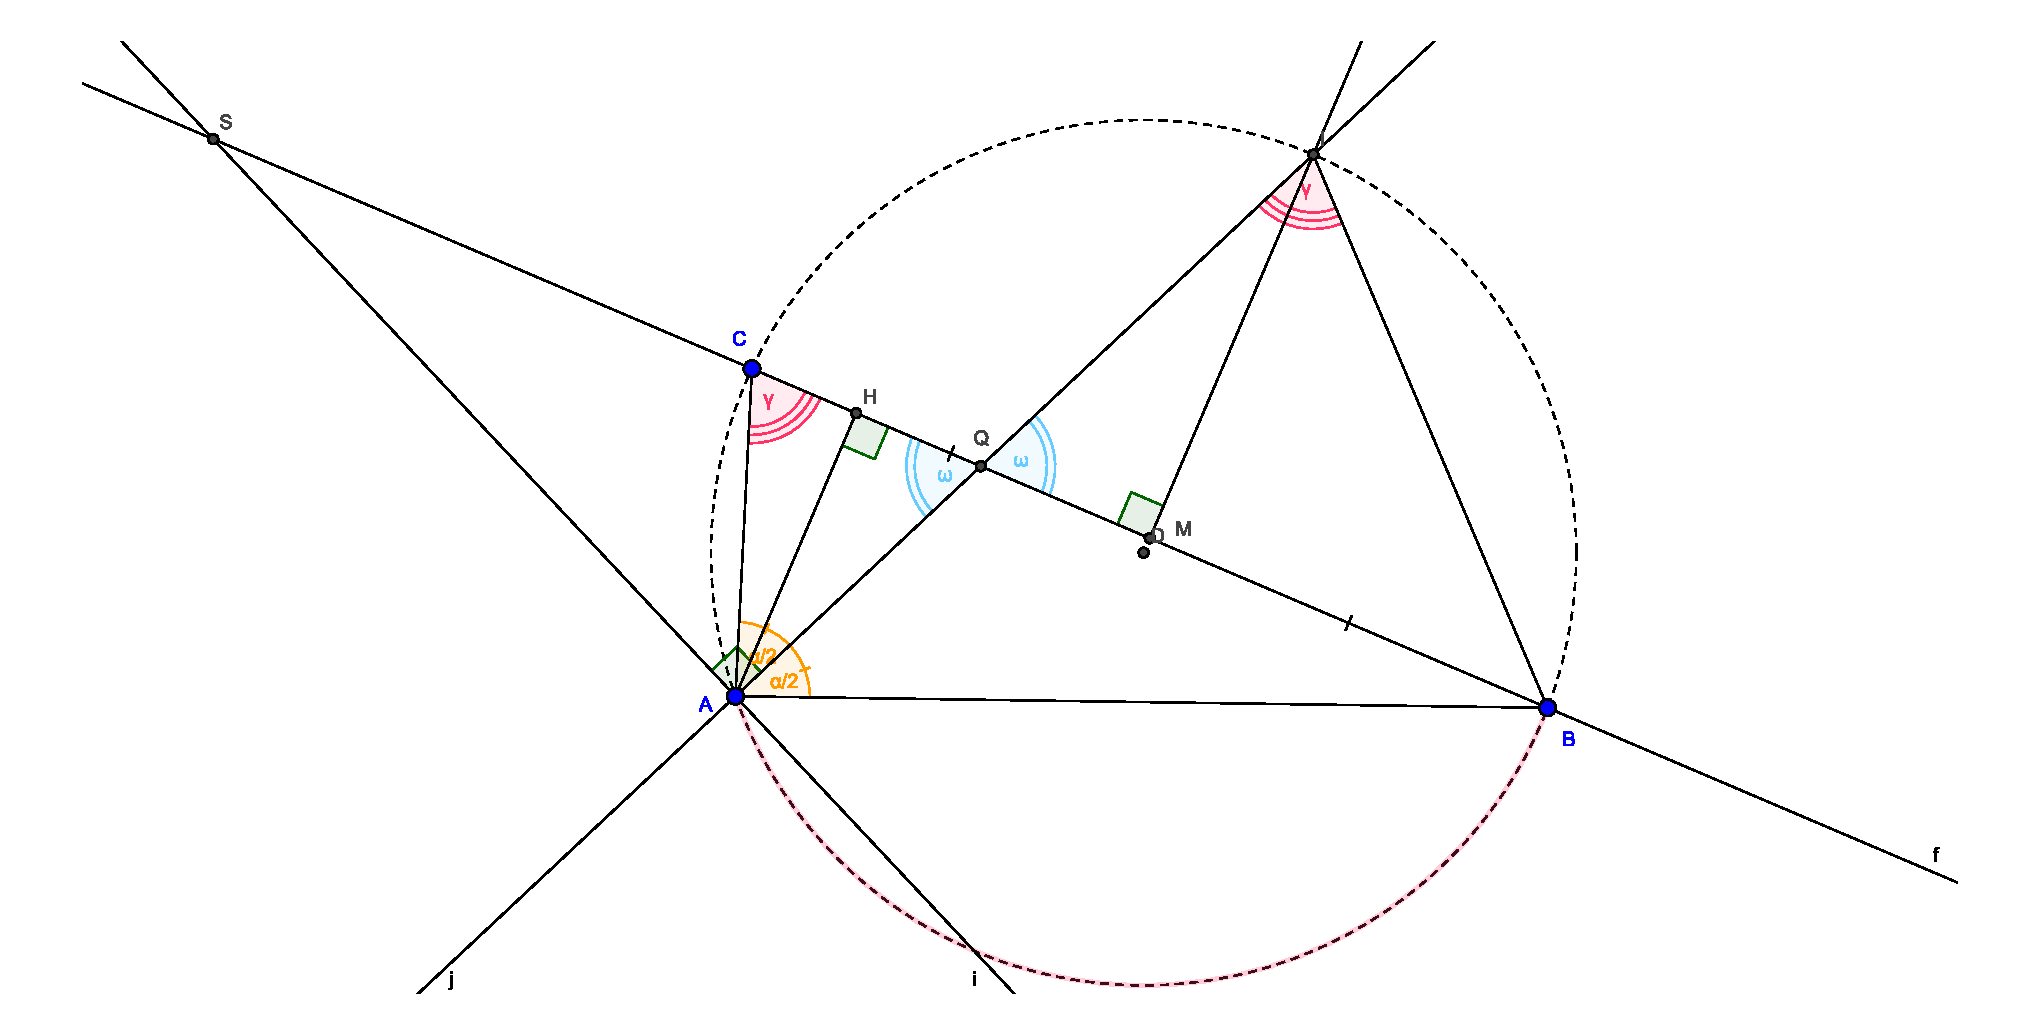
\includegraphics[width=\textwidth, trim=3cm 3cm 6cm 1.5cm, clip=true]{graphics/2016_8.pdf}

Par ailleurs, comme $\angle IMQ=\angle QAS=\angle AHQ=90^{\circ}$ et $\angle MQI=\angle HQA=\angle SQA$, on a que les triangles $MQI$, $AQS$ et $HQA$ sont semblables. Par conséquent,
\[
\frac{AQ}{HQ}=\frac{QI}{QM}=\frac{QS}{AQ}
\]
De cette égalité on déduit que
\[
\frac{AI}{MH}=\frac{AQ+QI}{HQ+QM}=\frac{QS}{AQ}
\]
puis que 
\begin{equation}
MH \cdot QS=AI \cdot AQ \label{eq:deux}
\end{equation}
L'énoncé suit alors directement de \eqref{eq:un} et \eqref{eq:deux}.

\textit{Marking Scheme:}
\begin{itemize}
	\item 1 Punkt dass $I$ auf dem Umkreis von $ABC$ ist.
	\item 2 Punkte für $QS \cdot MH = AQ \cdot AI$
	\item 1 Punkt für $\triangle AQB ~ \triangle ACI$
	\item 1 Punkt für $AQ \cdot AI = AB \cdot AC$
\end{itemize}

\newpage

\item[\textbf{9.}] %% Exercise 9 %%
Finde alle Funktionen $f\colon \R \to \R$, sodass für alle $x,y\in\R$ gilt:
\[
(f(x)+y)(f(x-y)+1)= f(f(xf(x+1)) - yf(y-1)).
\]

\textit{Lösung (Paul):}
Sei $x = 0, y = 1$:
\[
(f(0) + 1)(f(-1) + 1) = f(0).
\]
Setzen wir $y = -f(x)$, folgt sofort, dass ein $a \in \R$ existiert mit $f(a) = 0$. Nun setzen wir $x = a, y = 0$:
\[
0 = f(f(af(a + 1))).
\]
Und nun $x = a, y = a + 1$:
\[
(a + 1)(f(-1) + 1) = f(f(af(a + 1))) = 0.
\]
Wäre $a = -1$ würde die erste Gleichung $f(0) + 1 = f(0)$ liefern, ein Widerspruch. Folglich ist $a + 1 \neq 0$, sodass aus der letzten Gleichung $f(-1) = -1$ folgt. Setzen wir dies in der ersten Gleichung ein, folgt sofort $f(0) = 0$. Für $x$ setzen wir jetzt nacheinander $0$ und $-1$ ein, sodass gilt:
\[
yf(-y) + y = f(-yf(y-1)) = (y - 1)(f(-1 -y) + 1) \iff yf(-y) + f(-1 - y) + 1 = yf(-1 - y).
\]
Ersetzen wir hier $y$ durch $-y$, erhalten wir die Form:
\[
yf(y) = yf(y - 1) + f(y - 1) + 1.
\]
Jetzt setzen wir in der Originalgleichung nacheinander $y = 0, y = 1$ ein:
\[
f(x)^2 + f(x) = f(f(xf(x + 1))) = (f(x) + 1)(f(x -1) + 1) \iff f(x)^2 = f(x)f(x - 1) + f(x - 1) + 1.
\]
Wir ziehen nun die letzten beiden erhaltenen Gleichungen voneinander ab und erhalten:
\[
f(x)^2 - xf(x) = f(x)f(x - 1) - xf(x-1) \iff (f(x) - x)(f(x) - f(x - 1)) = 0.
\]
Können wir also für alle reellen $x$ zeigen, dass $f(x) \neq f(x - 1)$ gilt, folgt $f(x) = x$ und wir sind fertig. Dafür genügt es, Injektivität zu zeigen.

Sei $a$ wieder eine beliebige Nullstelle von $f$. Setze in der Originalgleichung $x = 0, y = a + 1$:
\[
(a + 1)(f(-a - 1) + 1) = 0,
\]
also mit der gleichen Argumentation wie vorher $f(-a - 1) = -1$. Sei nun $x = 0, y = -a$:
\[
-a = f(af(-a - 1)) = f(-a).
\]
Dann folgt mit $x = -1, y = -a$:
\[
(-1 - a)(f(a - 1) + 1) = f(af(-a - 1)) = f(-a) = -a \iff f(a - 1) = \frac{-1}{1 + a},
\]
da $a \neq -1$ ist. Dann gilt für $x = a - 1, y = 0$:
\[
\frac{1}{(a + 1)^2} - \frac{1}{a + 1} = 0 \iff a = 0.
\]
Folglich ist $0$ die einzige Nullstelle  von $f$, das heisst $f$ ist injektiv bei $0$.

Mit $y = -f(x)$ folgt dann:
\[
0 = f(f(xf(x + 1)) + f(x)f(-f(x) - 1)) \implies f(xf(x + 1)) = -f(x)f(-f(x) - 1)
\]
aufgrund der Injektivität bei $0$. Mit $x = y - 1$ folgt:
\[
0 = f(f((y - 1)f(y)) - yf(y-1)) \implies f((y - 1)f(y)) = yf(y - 1) \iff f(yf(y + 1)) = (y + 1)f(y),
\]
wenn wir $y$ durch $y + 1$ ersetzen, wobei wir wieder Injektivität bei $0$ benutzt haben. Ein Vergleich der letzten beiden Gleichungen liefert:
\[
(y + 1)f(y) = -f(y)f(-f(y) - 1).
\]
Für $y \neq 0$ können wir $f(y)$ wegkürzen und es bleibt $f(-f(y) - 1) = -y - 1$, was sogar für $y = 0$ auch stimmt. Mit dieser Gleichung können wir nun Injektivität zeigen. Sind $u, v \in \R$ mit $f(u) = f(v)$, gilt
\[
-u - 1 = f(-f(u) - 1) = f(-f(v) - 1) = -v - 1 \implies u = v,
\]
wie gewünscht. Also sind wir fertig.

Einsetzen zeigt, dass $f(x) = x$ wirklich eine Lösung ist.

\textit{Marking Scheme:}
\begin{itemize}
	\item 1 Punkt für $f(0) = 0$
	\item 2 Punkte für Injektivität bei $0$
	\item 1 Punkt für Injektivität auf ganz $\mathbb{R}$
	\item 2 Punkte für $f(x)^2 - xf(x) = f(x)f(x - 1) - xf(x-1)$, 1 weiterer für die Faktorisierung
\end{itemize}

\newpage

\item[\textbf{10.}] %% Exercise 10 %%
Soit $ABC$ un triangle non-rectangle avec $M$ le milieu de $BC$. Soit $D$ un point sur la droite $AB$ tel que $CA=CD$ et soit $E$ un point sur la droite $BC$ tel que $EB=ED$. La parallèle à $ED$ passant par $A$ coupe la droite $MD$ au point $I$ et la droite $AM$ coupe la droite $ED$ au point $J$. Montrer que les points $C$, $I$ et $J$ sont alignés.

\textit{Lösung (Horace):}
Soit $P$ le milieu de $AD$. Par propriété des triangle isocèle on a que le milieu de la base est égal au pied de la hauteur issue du sommet opposé à la base. L'utilisation de cette propriété dans le triangle par construction isocèle en $C$ $ACD$, on a que $\angle CPD=90^{\circ}$. Par la réciproque du théorème des cercles de thalès dans le triangle rectangle $CPB$ on a que $C$, $P$ et $B$ sont sur un cercle de centre $M$. On a en particulier $MP=MB$. Par conséquent $PMB$ est isocèle en $M$ et ainsi $\angle BPM=\angle PBM$. Dans le triangle par construction isocèle en $E$ $BED$ on a que $\angle EDB=\angle EBD$. Comme $\angle EBD=\angle PBM$ on a que $\angle BPM=\angle PBM=\angle EBD=\angle BDE$. Par conséquent $PM$ est parallèle à $ED$. On a donc que les segment $PM$, $ED$, $AI$, $DJ$ sont tous parrallèle entre eux. Les triangle $AMP$ et $AID$ (1), $DMP$ et $DIA$ (2) sont donc par thalès semblables avec un facteur de proportionalité de $2$ car $\frac{DA}{DP}=\frac{AD}{AP}=2$. Soient $I'$, $M'$ et $J'$ les projections de $I$, $M$, resp. $J$ sur $AB$. Comme $\angle BM'M=\angle BPC= 90^{\circ}$, comme $\angle M'BM=\angle PMC$, on a que $M'MB$ est semblable à $PCB$ avec un facteur de proportionalité de $2$ car $\frac{CB}{MB}=2$ (3).
Nous utiliserons sans précision dans la suite des cacules que le facteur de proportionalité entre les longueurs des cotés de deux triangle semblables est le même que le facteur de proportionalité entre les longueurs des hauteurs correspondantes.

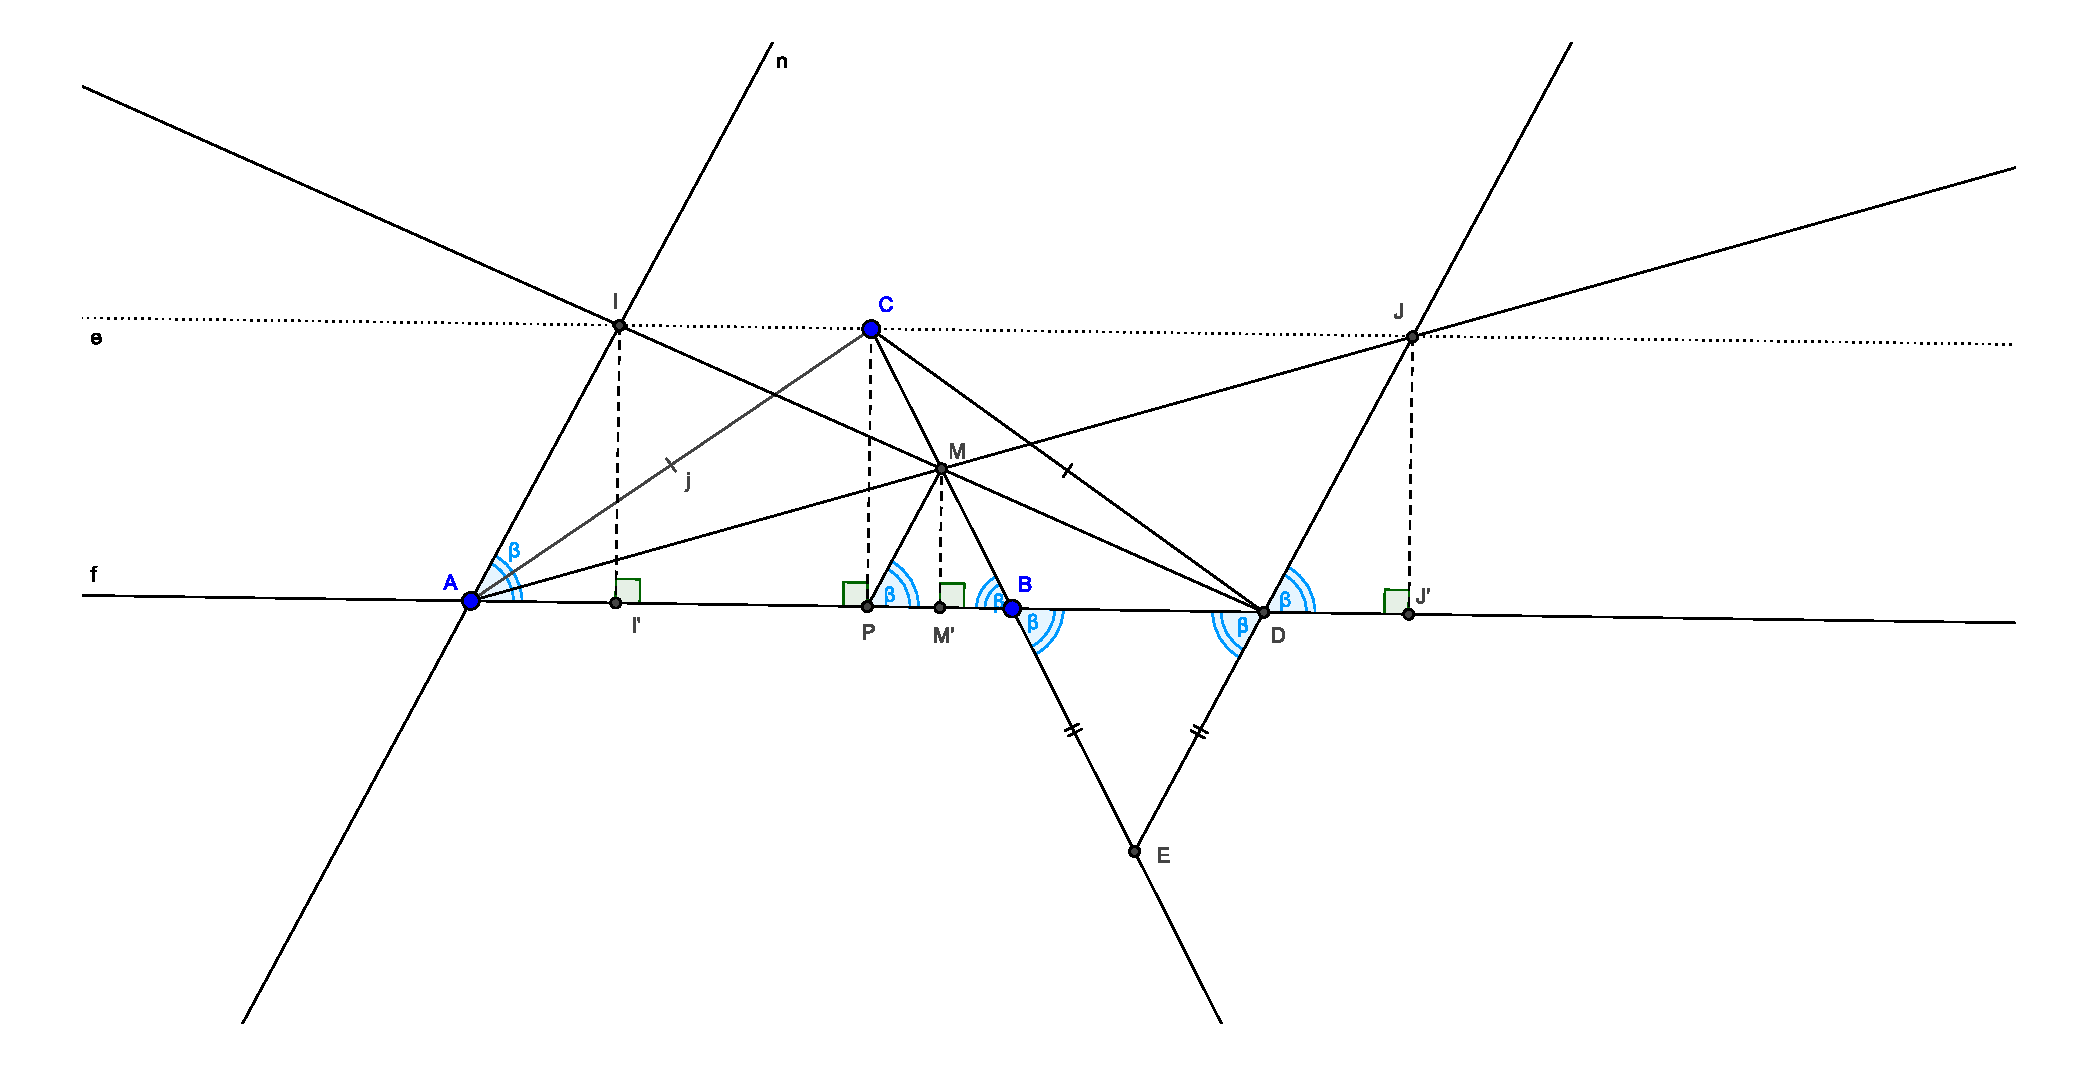
\includegraphics[trim=7cm 3cm 9cm 3cm, clip=true, width=\textwidth]{graphics/2016_10}

Par (1), (2) et (3), on a que 
\[
II'=2MM'=CP=2MM'=JJ'
\]
Par ailleurs, on a 
\[
\angle II'P=\angle CPI'=\angle CPJ'=\angle PJ'J=90^{\circ}
\]
De là s'ensuit que les quadrilatère $II'PC$ et $CPJ'J$ sont des rectangles. Ainsi
\[
\angle ICJ=\angle ICP+\angle PCJ=90^{\circ}+90^{\circ}=180^{\circ}
\]
Ce qui termine la preuve.

\textit{Marking Scheme}
\begin{itemize}
	\item 2 points pour avoir trouvé une relation entre $M$ et $I$ ou entre $M$ et $J$.
	\item 3 points pour avoir trouvé une relation entre $M$ et $I$ et entre $M$ et $J$.
	\item 1 point pour avoir trouvé une relation interessante avec $M$.
	\item 1 point pour trouvé que $AB$ est parrallèle à $IC$ ou à $CJ$.
\end{itemize}


\newpage

\item[\textbf{11.}] %% Exercise 11 %%

Seien $m$ und $n$ natürliche Zahlen mit $m>n$. Definiere
\[
x_k = \frac{m+k}{n+k}\text{ für }k=1, \ldots, n+1.
\]
Zeige: Wenn alle $x_i$ ganzzahlig sind, ist $x_1\cdot x_2 \cdot \ldots \cdot x_{n+1} - 1$
keine Zweierpotenz.

\textit{Lösung 1:}
Nehme an, dass $x_1, x_2, \ldots ,x_{n+1}$ ganze Zahlen sind. Definiere die Zahlen 
\[
a_k=x_k -1= \frac{m+k}{n+k}-1= \frac{m-n}{n+k}>0
\]
für $k=1,2,\ldots ,n+1$.\\
Sei $P=x_1x_2\ldots x_{n+1}-1$. Wir betrachten, welche  Zweierpotenzen die natürlichen Zahlen $a_k$ teilen. \\
Sei $2^d$ die grösste Zweierpotenz, welche $m-n$ teilt, und $2^c$ die grösste Zweierpotenz kleiner  gleich $2n+1$. Dann gilt $2n+1\leq2^{c+1}-1$, und damit $n+1\leq2^c$. Wir folgern, dass  $2^c$ eine der Zahlen $n+1, n+2, \ldots ,2n+1$ ist und keine andere dieser Zahlen durch $2^c$ teilbar ist. Wähle $l$, sodass $n+l=2^c$. Da $\frac{m-n}{n+l}$ eine ganze Zahl ist, gilt $d\geq c$. Also gilt $2^{d-c+1}\ndiv a_l=\frac{m-n}{n+l}$, und $2^{d-c+1} \div a_k$ für alle $k \in \{1,\ldots,n+1\}\setminus \{l\}$.

Nun gilt:
\[
P=(a_1+1)(a_2+1)\cdots(a_{n+1}+1)-1\equiv(a_l+1)\cdot1^n-1\equiv a_l\nequiv 0 \pmod{2^{d-c+1}}.
\]
Also gilt $2^{d-c+1}\ndiv P$.

Andererseits gilt für alle $k\in \{1,\ldots,n+1\}\setminus\{l\}$, dass  $2^{d-c+1}\div a_k$. Somit gilt $P\geq a_k\geq2^{d-c+1}$, und ist somit keine Zweierpotenz. 

\textit{Lösung 2:}
Wir suchen einen ungeraden Teiler grösser 1 von $P$. Da $a_k\in \N$, ist $m-n$ teilbar durch $n+1, n+2, \ldots, 2n+1$, und somit auch durch ihren kleinsten gemeinsamen Teiler $L$. Also gilt $m-n=qL$ für eine natürliche Zahl $q$, und $x_k=q\cdot\frac{L}{n+k}+1$.\\
Weil $n+1\leq 2^c=n+l\leq2n+1\leq2^{c+1}-1$, gilt $2^c\div L$ und $2^{c+1}\ndiv L$. Also ist $\frac{L}{n+l}$ ungerade und $\frac{L}{n+k}$ gerade für alle $k\neq l$. Nun gilt:
\[
P=x_1x_2\cdots x_{n+1}-1\equiv(q+1)\cdot1^n-1\equiv q \pmod{2q}
\]
Also gibt es eine natürliche Zahl $r$ mit $P=x_1x_2\cdots x_{n+1}-1\geq2qr+q=q(2r+1)$.
Weil $P=x_1x_2\cdots x_{n+1}-1\geq x_1x_2-1\geq(q+1)^2-1>q$, gilt $r\geq1$. Und somit ist $P$ durch eine ungerade Zahl teilbar.

\textit{Marking Scheme:}
\begin{itemize}
	\item In den Zahlen $n,\ldots 2n+1$ kommt die grösste Zweierpotenz nur einmal vor oder $L=\kgV(n,\ldots,2n+1)$ teilt $m-n$ und nur eine der Zahlen $L/(n+i)$ ist ungerade. 2 Punkte.
	\item Sinnvoll modulo rechnen bezüglich etwas Sinnvollem. 3 Punkte.
\end{itemize}


\newpage

\item[\textbf{12.}] %% Exercise 12 %%
An einer EGMO-Prüfung gibt es drei Aufgaben, wobei bei jeder Aufgabe eine ganzzahlige Punkt\-zahl zwischen 0 und 7 erreicht werden kann. Zeige, dass es unter 49 Schülerinnen immer zwei gibt, sodass die eine in jeder der drei Aufgaben mindestens so gut war wie die andere.

\textit{Lösung 1 (Cyril):}
Wir nehmen an, dass wir möglichst viele Schülerinnen haben, sodass wir keine zwei finden, die die Voraussetzung erfüllen. Wir zeigen, dass es dann maximal 48 Schülerinnen geben kann.

Wir teilen die Schülerinnen in bis zu 8 Gruppen ein gemäss der Punktzahl der ersten Aufgabe. Sei $a_i$ die Grösse der Gruppe mit $i$ Punkten bei der ersten Aufgabe.

\textbf{Beobachtung 1:} Innerhalb einer Gruppe ist die Punkteverteilung der zweiten und dritten Aufgabe genau invertiert. Dies daher, da der schlechteste der zweiten Aufgabe der beste der dritten Aufgabe sein muss, gleichermassen für den zweitschlechtesten.

\textbf{Definition:} Wir nennen die Resultate einer Gruppe \emph{fast optimal}, wenn alle die selbe Gesamtpunktzahl erreicht haben. Wir nennen sie \emph{optimal}, wenn alle dafür möglichen Kombinationen vorkommen.

\textbf{Beobachtung 2:} Ist eine Gruppe optimal angeordnet, dann würde eine Schülerin aus einere besseren Gruppe genau dann die Voraussetzung erfüllen, wenn sie in der zweiten und dritten Aufgabe insgesamt mehr Punkte gemacht hätte. Das heisst es gibt in besseren Gruppen eine kritische Punktzahl, die nicht überschritten werden darf.

Wir zeigen, dass wir bei möglichst vielen Schülern alle Gruppen optimal anordnen können.

\textbf{Induktionsansatz:} Wir beginnen nun bei der Gruppe mit 0 Punkten bei der ersten Aufgabe. Diese können wir optimal anordnen, indem wir die Punktzahlen bei der zweiten und dritten Aufgabe erhöhen, bis in beiden Aufgaben die Punktzahlen $7,6, \ldots, 7-a_0+1$ erreicht sind. Da diese Gruppe in der ersten Aufgabe am schlechtesten war, haben wir auch keinen Widerspruch erzeugt, indem wir Punktzahlen erhöht haben.

\textbf{Induktionsschritt:} Wir betrachten die nächste Gruppe. Wir können diese sicher fast optimal anordnen: Wir suchen eine Schülerin, die nicht das Gruppenmaximum erreicht hat. Diese muss in einer Aufgabe weniger als 7 Punkte erreicht haben, sagen wir sie hat $p$ erreicht. Falls $p+1$ von niemandem erreicht wurde, können wir ihre Punktzahl auf $p+1$ erhöhen. Andernfalls hat es eine Schülerin, die $p+1$ Punkte erreicht hat. Diese hat sicher auch nicht das Punktmaximum erreicht, da sie in der anderen Aufgabe strikt weniger Punkte gemacht haben muss. Wir können also mit ihr weiterfahren. Entweder ist $p+2$ belegt oder wir können ihre Punktzahl erhöhen. Wenn wir so weiter machen und die Punktzahl nie erhöhen können, muss die beste von dieser Aufgabe auch nicht das Gruppenmaximum erreicht haben. Jetzt können wir aber das gleiche Spiel mit der anderen Aufgabe machen, wo sie am schlechtesten sein muss. Entweder wir können eine Punktzahl erhöhen oder alle bis und mit der besten hat nicht die Gesamtpunktzahl erreicht. Dann hätten aber niemand das Maximum erreicht, Widerspruch. Also können wir immer jemandem mehr Punkte geben, bis alle gleich viel haben.

Ist die Gruppe nun erst fast optimal, dann fügen wir neue Schülerinnen hinzu, die die fehlenden Kombinationen von Punkten erreicht haben. Vielleicht müssen wir diese aus späteren Gruppen wegnehmen, aber wir verringern die Anzahl Schülerinnen sicher nicht.

Damit können wir alle Gruppen optimal anordnen, ohne die Anzahl Schülerinnen zu verringern. Die zur Verfügung stehenden Gruppengrössen sind: $1,2,3,4,5,6,7,8,7,6,5,4,3,2,1$. Da es maximal 8 Gruppen gibt, ist das Maximum von Schülerinnen: $8+7+7+6+6+5+5+4=48$.

\newpage

\textit{Lösung 2 (Cyril):}

Wir betrachten die Resultate der ersten beiden Aufgaben und teilen diese so in Gruppen auf, dass keine zwei aus einere Gruppe das gleiche Resultat bei der letzten Aufgabe haben dürfen.

Wir bezeichnen mit $(a,b)$ das Resultat, in der ersten Aufgabe $a$ Punkte und in der zweiten $b$ Punkte zu haben. Die Gruppen sind dann:
\[
(0,0), (0,1), (0,2), (0,3), (0,4), (0,5), (0,6), (0,7), (1,7), (2,7), (3,7), (4,7), (5,7), (6,7), (7,7)
\]  
\[
(1,0), (1,1), (1,2), (1,3), (1,4), (1,5), (1,6), (2,6), (3,6), (4,6), (5,6), (6,6), (7,6)
\]
\[
(2,0), (2,1), (2,2), (2,3), (2,4), (2,5), (3,5), (4,5), (5,5), (6,5), (7,5)
\]
\[
(3,0), (3,1), (3,2), (3,3), (3,4), (4,4), (5,4), (6,4), (7,4)
\]
\[
(4,0), (4,1), (4,2), (4,3), (5,3), (6,3), (7,3)
\]
\[
(5,0), (5,1), (5,2), (6,2), (7,2)
\]
\[
(6,0), (6,1), (7,1)
\]
\[
(7,0)
\]

Graphisch dargestellt:
\begin{center}
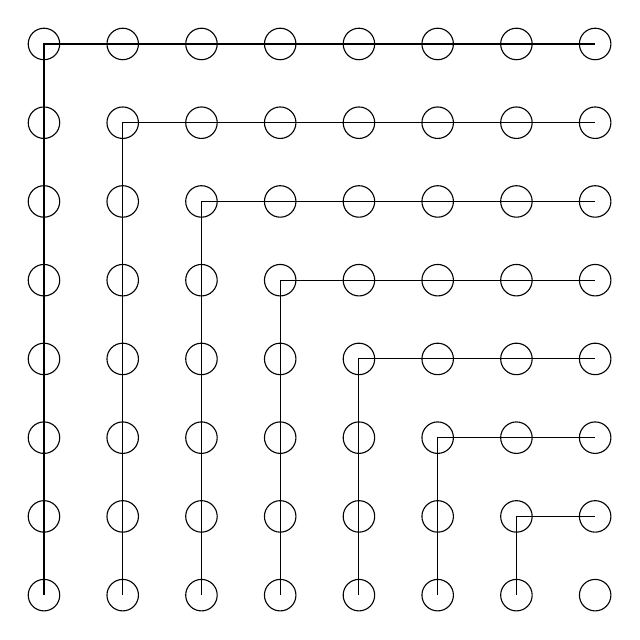
\begin{tikzpicture}[main node/.style={circle, fill=blue!20, draw}]
\draw (0,0) -- (0,1) -- (0,2) -- (0,3) -- (0,4) -- (0,5) -- (0,6) -- (0,7) -- (1,7) -- (2,7) -- (3,7) -- (4,7) -- (5,7) -- (6,7) -- (7,7);
\draw (1,0) -- (1,1) -- (1,2) -- (1,3) -- (1,4) -- (1,5) -- (1,6) -- (2,6) -- (3,6) -- (4,6) -- (5,6) -- (6,6) -- (7,6);
\draw (2,0) -- (2,1) -- (2,2) -- (2,3) -- (2,4) -- (2,5) -- (3,5) -- (4,5) -- (5,5) -- (6,5) -- (7,5);
\draw (3,0) -- (3,1) -- (3,2) -- (3,3) -- (3,4) -- (4,4) -- (5,4) -- (6,4) -- (7,4);
\draw (4,0) -- (4,1) -- (4,2) -- (4,3) -- (5,3) -- (6,3) -- (7,3);
\draw (5,0) -- (5,1) -- (5,2) -- (6,2) -- (7,2);
\draw (6,0) -- (6,1) -- (7,1);
\draw (7,0);
\foreach \x in {0,...,7}
\foreach \y in {0,...,7} 
  \draw (\x,\y) circle (0.2);
\end{tikzpicture}
\end{center}

Die Grössen dieser Gruppen sind $1,3,5,7,9,11,13,15$ wobei wir maximal 8 aus einer Gruppe wählen können. Wir können also maximal $1+3+5+7+8+8+8+8=48$ Teilnehmerinnen wählen.

\textit{Marking Scheme:}
\textit{Lösung 1}
2 Punkte für das Aufteilen aller möglichen Resultate in acht Gruppen, sodass für je zwei Schülerinnen in einer Gruppe, die eine in den ersten zwei Aufgaben jeweils mindestens so viele Punkte wie die andere hat.

\textit{Lösung 2}
Bis zu 4 Punkte für Lösungsansätze, welche die Aufgabe vereinfachen und sich zu einer Lösung vervollständigen lassen.

\end{enumerate}

\end{document}
